\section{Optimising Extended Feature Models}\label{sec:tools}
In the introduction, we introduced the concept of \emph{optimising}
products in software product lines. This optimisation process involves
at least one objective, in case of multiple objectives, the problem is
called a \emph{multi-objective} optimisation problem. Optimisation can only be done
in \emph{Extended Feature Models}, as they contain the relevant data
to optimise on. We know that the optimisation is NP-complete, as we want
to optimise multiple orthogonal objectives~\cite{ochoa2018npcomplete}.
A multitude of tools has been created in the past to try to solve the
optimisation problem. The most successful tools rely on genetic algorithms,
specifically the IBEA algorithm~\cite{zitzler2004ibea}. We are not going
to introduce the idea of genetic algorithms to the fullest extent here,
for more background into those, we refer you to for
example~\cite{kramer2017geneticalgos}. The basic idea is that we can
encode solutions in for example a binary bitstring. The algorithm can then
create new solutions by mutating the bitstrings (a mutation operator) and
by combining two bitstrings into one or more new solutions (a crossover 
operator). In the optimisation problem of products in software product lines,
solutions are often encoded using bitstrings as well. In those bitstrings,
a \texttt{1} represents a feature that is enabled, and a \texttt{0} 
represents a disabled feature. As long as we keep the ordering of the
features fixed, we can fully describe products using this bitstring.
In this section, we will look at how some of the state-of-the-art tools work
in more detail. We will first look at MODAGAME~\cite{pascual2015modagame}
and then look into aCaPulCO~\cite{horcas2022breakit} in even more detail, as 
we will also be working with this tool. The tools that we are talking about
are all based on the IBEA genetic algorithm, so we focus on those.

\subsection{MODAGAME}\label{sec:modagame}
Before we delve into how a tool such as MODAGAME~\cite{pascual2015modagame}
works exactly, we should take a look at the general way how these tools
function.

In genetic algorithms, we have three important phases: we first need to
select parents to create new offspring with (the \emph{selection} process),
then we create new offspring in the \emph{crossover} process, and finally
we make slight adjustments to the offspring in the \emph{mutation} process.
As mentioned before, the products are represented using bitstrings where
each bit is a feature that can be enabled (\texttt{1}), or disabled 
(\texttt{0}).

\textit{Selection} The selection process is not the most relevant
to look at for our work, the process is usually done by some standard
selection such as Binary Tournament Selection, where two individuals are
compared and the best of the two individuals is selected.

\textit{Crossover} The crossover operator should combine several parents
(usually two), to create new offspring. We can of course have multiple
different parents and children, depending on the type of crossover that we
choose. In a simple implementation such as \emph{Single-Point Crossover}, we
choose a location in the bitstring and split the (two) parents at that
location. We can then create new children by combining the bitstrings from
the first and second parents. Crossover happens at a probability decided by a 
parameter.

\textit{Mutation} A mutation operator creates more variability in the 
offspring created by the crossover operator. The mutation operator on a bitstring
can be implemented trivially. For each bit in the bitstring, we can flip each bit
at a given probability.

These three steps in a genetic algorithm work well for optimising feature models.
There is a problem, however, the simple implementation of the operators does not
keep into account the limitations we have previously put on the relations of features.
We can have for example some mandatory feature that might be disabled by a mutation
operator. Where keeping into account mandatory features is (relatively) simple,
we know that Cross-Tree constraints can contain any generic boolean formula. 
Keeping these into account during the crossover and mutation processes is very
expensive.

\textit{Fix operator} MODAGAME~\cite{pascual2015modagame} keeps these restrictions
into account in different ways. The most relevant and interesting way for us is the
\emph{fix} operator. This is another operator besides the selection, crossover and
mutation operators. It is executed after initialising solutions and after creating
new offspring. The idea of the \emph{fix} operator is that invalid representations
can be fixed during this process. One can imagine that this fixing of constraints
is expensive. In the results of MODAGAME, it is also made clear that the \emph{fix}
operator takes most of the time of the overall runtime in large feature models
(around 80\% to 90\% of the runtime.) In MODAGAME, the cross-tree constraints are
handled separately from the other constraints on the tree (such as XOR- or OR-groups).
The group constraints are repaired by enabling disabled features in an allowed manner
(i.e. by adhering to the defined groups), this is an expensive recursive operation
where enabling one feature might even lead to checking all other features. This process
will always result in a configuration that is valid to the group constraints.

The process for repairing the cross-tree constraints is different, as it is not always
guaranteed to succeed. Cross-tree constraints are often represented in CNF, where
each boolean formula is written as a conjunction of disjunctions. The \emph{fix}
operator attempts to fix invalid cross-tree constraints by attempting to fix each
disjunction separately. To fix a disjunction, we need to make one of the literals
in the disjunction positive. MODAGAME does this in a random order such that different
features are enabled every time (to increase the chance of success). Enabling the
feature is done using the same function that is used in the fixing of the group
constraints, such that enabling this feature does not break other group constraints.
It may, however, happen that other cross-tree constraints are no longer satisfied when
one of them is repaired. For this reason, the entire process of repairing cross-tree
constraints need to be restarted each time a fix is applied. This makes the repair
process for cross-tree constraints even more expensive than the previous repair process.

\subsection{aCaPulCO}\label{sec:acapulco}
Now that we have looked at how MODAGAME works, we can take a look at the tool that
we will be working with in more detail: aCaPulCO~\cite{horcas2022breakit}. The goal
of aCaPulCO was to remove the need for the \emph{fix} operator, as it slows down
the optimisation process the most. Besides slowing down the process, it also yields
incorrect solutions as the aforementioned \emph{fix} operator of MODAGAME sometimes
fails to fix the cross-tree constraints. By design, aCaPulCO does not create any
incorrect products. This section covers more details of aCaPulCO, how it works,
and also what its shortcomings are.

\emph{CPCOs} The underlying system of aCaPulCO relies on so called
\emph{Consistency-preserving configuration operators} (CPCOs). These operators
allow enabling or disabling features without breaking any constraints of the
underlying feature model. Unlike other tools, aCaPulCO can calculate these static
operators before executing the analysis part of the tool. This means that for
every feature model, the operators to enable and disable features only have to be
computed once. 

There are some principles on which the CPCO generation relies, six for the
activation of features (\emph{Activation principles}), and five for the
deactivation of features (\emph{Deactivation principles}). These are as follows
for the activation principles, where $f$ is a feature that we want to activate:
\begin{enumerate}
    \item \textsc{ActMand}: Activate all mandatory children of $f$.
    \item \textsc{ActPar}: If $g$ is the parent of $f$, and it is not activated, activate $g$.
    \item \textsc{ActReq}: If $f$ requires feature $g$, and it is not actiated, activate $g$.
    \item \textsc{ActGroup}: If $f$ is an \emph{OR} or \emph{XOR} group, activate one of the children of $f$.
    \item \textsc{ActXor}: If $f$ is one of the children of an \emph{XOR} group, deactivate all of the siblings of $f$.
    \item \textsc{ActExc}: If $f$ is excluded by, or excludes $g$, deactivate $g$.
\end{enumerate}

For the deactivation principles, we have the following, where $f$ is the feature
to be deactivated:
\begin{enumerate}
    \item \textsc{DeChild}: Deactivate all active children of $f$.
    \item \textsc{DeXor}: If $f$ is one of the children of an \emph{XOR} group, either activate one of the siblings of $f$, or deactivate its parent.
    \item \textsc{DeOr}: If $f$ is one of the children of an \emph{OR} group, either activate one of its siblings or deactivate the parent of $f$.
    \item \textsc{DeParent}: If $f$ is a mandatory feature, deactivate the parent of $f$.
    \item \textsc{DeReq}: If a feature $g$ requires $f$, deactivate $g$.
\end{enumerate}

Note that we are talking about \emph{requires} and \emph{excludes} relationships.
It should be noted that these kinds of constraints are located in the cross-tree
constraints, but these constraints are of certain shapes. The aCaPulCO tool
currently only accepts cross-tree constraints that define some requirement of a
feature (e.g. feature $f$ \emph{requires} feature $g$), or an exclusion of a
feature (e.g. feature $f$ cannot be activated when feature $g$ is active: 
$g$ \emph{excludes} $f$). In aCaPulCO, we differentiate between these constraints
(we refer to them as \emph{simple} constraints), and constraints of other shapes,
which we refer to as \emph{complex} constraints. Note that these constraints are
only relevant in the cross-tree constraints.

With the previously defined principles, we can generate sound activation and
deactivation rules for all of the features. One problem with generating the 
rules naively with just these constraints is not scalable to large feature models,
which are specifically the target of aCaPulCO. This is why an efficient algorithm
is defined for generating the CPCOs in~\cite{horcas2022breakit}. We will not cover
this algorithm in detail as it is not relevant to our work.

\begin{figure}
    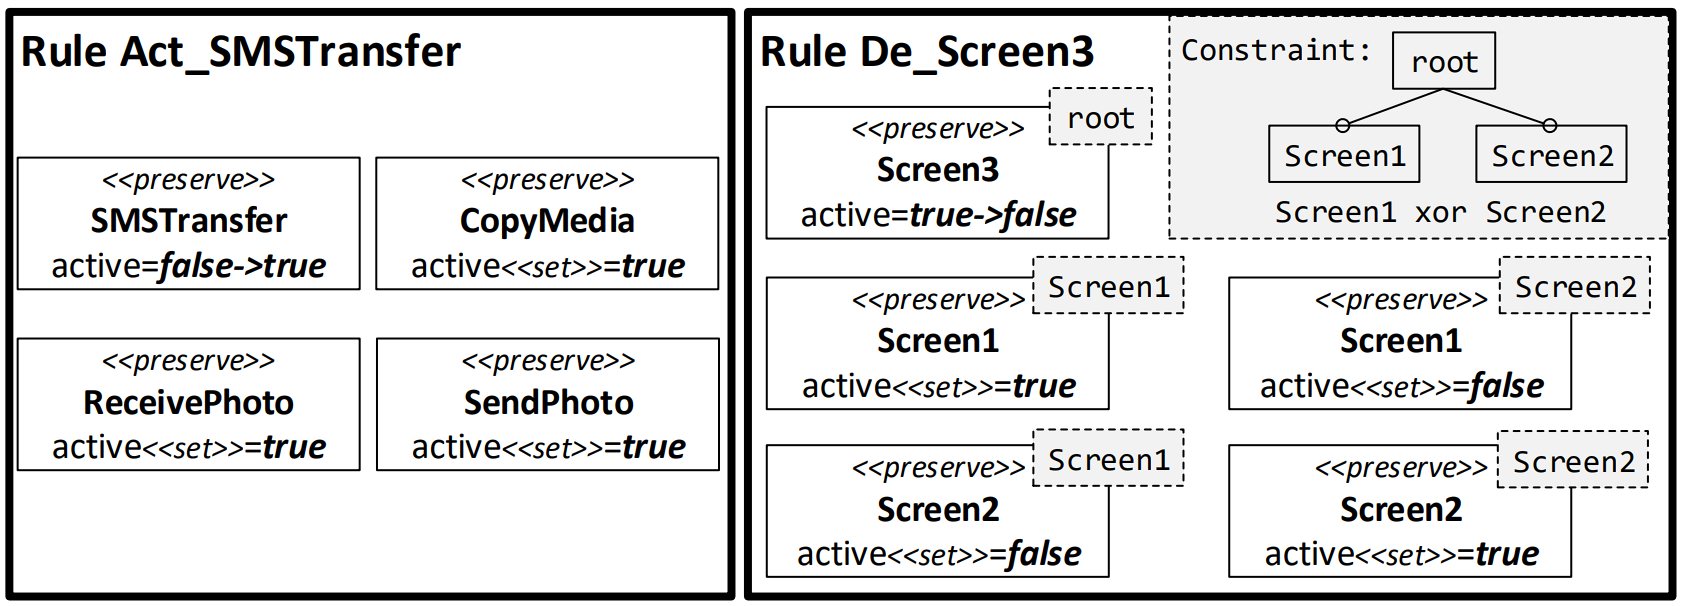
\includegraphics[width=\textwidth]{examplerules}
    \caption{Two example CPCOs for features \emph{SMSTransfer} and \emph{Screen3} of the feature model we have introduced in Figure~\ref{fig:example:mobilemedia}.}
    \label{fig:example:cpcos}
\end{figure}

Let us look at two example rules for the activation and deactivation of features
that we introduced in Figure~\ref{fig:example:mobilemedia}. We show the activation
of \emph{SMSTransfer} and the deactivation of \emph{Screen3} in 
Figure~\ref{fig:example:cpcos}. On the left, we can see the activation, where we set
\emph{SMSTransfer} to \emph{true} from \emph{false}. To do this, we also need to set
\emph{CopyMedia}, \emph{ReceivePhoto} and \emph{SendPhoto} to active. The deactivation
rule on the right is more complex. This is because the \emph{ScreenSize} feature is an
\emph{XOR} group that contains the three screen sizes. Since we want to deactivate
\emph{Screen3}, the remaining constraint is that exactly one of \emph{Screen1} and
\emph{Screen2} must be active. In the rule, we can see that we firstly set
\emph{Screen3} to \emph{false} from \emph{true}. Then we have two options, which we
label with either of the two remaining screen sizes. In one option, we enable
\emph{Screen1} and disable \emph{Screen2}, the other option is the inverse of this.

We previously mentioned how a difference is defined between two types of cross-tree constraints. We have the \emph{simple} cross tree constraints, with which
aCaPulCO can work (the CPCO generation can adhere to these rules). But we also
have \emph{complex} cross-tree constraints. The current version of aCaPulCO
cannot deal with these constraints. The reason for this is that the CPCO
generation gets too complex with the addition of these constraints. This is not
surprising, we have also seen this in MODAGAME, where the \emph{fix} operator 
will take increasingly more time when the size of the feature models is scaled
up.

To fix this, the authors of aCaPulCO already suggested going with a hybrid
approach (albeit such an approach has not been developed and implemented in
previous work): we keep the complex constraints out of the CPCO generation and only
take them into account in a \emph{fix} operator. This would mean that a new
processing step is added to aCaPulCO, in which only the complex constraints are
handled. Supposedly, this works better than MODAGAME, because that tool takes
care of all the types of cross-tree constraints in its \emph{fix} operator.

